\newcommand{\plB}{\plfoo{B}}
\newcommand{\plE}{\plfoo{E}}

\begin{frame}{}
	\begin{block} {Aussagenlogik}
	\begin{itemize}
		\item \enquote{Es regnet und alle Vögel sind grau.}
		\item atomar: \enquote{Es regnet.}, \enquote{ Alle Vögel sind grau.}
		\item Diese beiden Aussagen lassen sich ihrerseits nicht in weitere Teilaussagen zerlegen!
	\end{itemize}
	\end{block}

	\pause
	\begin{block} {Prädikatenlogik}	
		\begin{itemize}
		\item In der Prädikatenlogik werden atomare Aussagen hinsichtlich ihrer inneren Struktur untersucht.
		\item \enquote{Alle Vögel sind grau}
		\item lässt sich in : \enquote{Alle Vögel}, \enquote{sind grau} zerlegen.
	\end{itemize}
	
	\end{block}
\end{frame}

\section{Prädikatenlogik: Syntax}

\begin{frame}{Aufgabe 1 (15/16, Blatt 7)}
	  Es seien $\CPL = \{ \}$, $\VPL = \{ \plx, \ply, \plz \}$, $\FPL = \{ \}$ und $\RPL = \{ \plE, \pleq \}$ mit $\ar(\plE) = 2$, und es sei $F$ die prädikatenlogische Formel
	\begin{equation*}
	\alnot \plexist \plx
	{\plka
		\plE{\plka \plx \plcomma \ply \plkz}
		\alor
		\alnot \plall \plz \plall \plx \plall \ply
		{\plka
			\plE{\plka \plx \plcomma \plz \plkz} \aland \plE{\plka \ply \plcomma \plz \plkz} \alimpl \plx \pleq \ply
			\plkz}
		\plkz}
	\end{equation*}
	
	\begin{block}{Aufgabe 1.0}
	Ist diese prädikatenlogische Formel syntaktisch korrekt?\\ \pause
	Ja
	\end{block}
\end{frame}

\begin{frame}{Syntax}
	\begin{block}{Aufbau von prädikatenlogischen Formeln}
	\begin{itemize}[<+->]
		\item \textbf{Terme}: Liefern \enquote{Werte}; Aus Konstanten, Variablen und Funktionssymbolen zusammengesetzt.
		\item \textbf{Atomare Formeln}: Liefern \enquote{Wahrheitswerte}; Aus Termen und Relationssymbolen zusammengesetzt.
		\item \textbf{Prädikatenlogische Formeln}: Verknüpfen und Quantifizieren atomare Formeln; Aus atomaren Formeln und aussagenlogischen Konnektiven sowie Quantoren zusammengesetzt. 
	\end{itemize}
	\end{block}
\end{frame}


\begin{frame}{Terme - Alphabet}
\begin{figure}
	\centering
	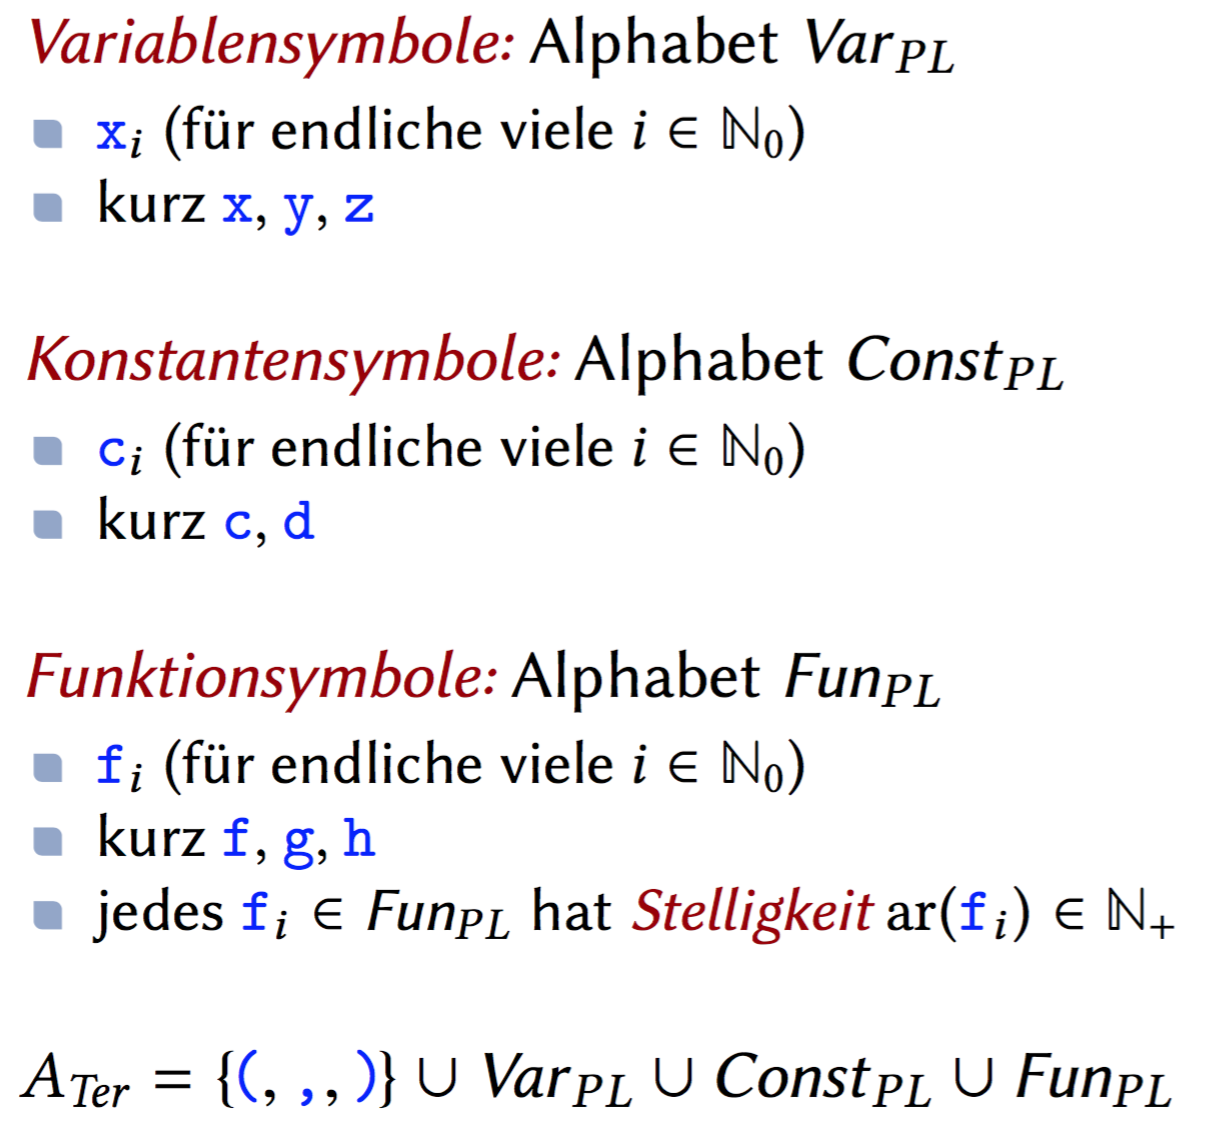
\includegraphics[scale=0.2]{pl/TermeAlphabet.png} \hspace{2em} 
\end{figure} 
\end{frame}

\begin{frame}{Terme - Grammatik}
\begin{figure}[h!]
	\centering
	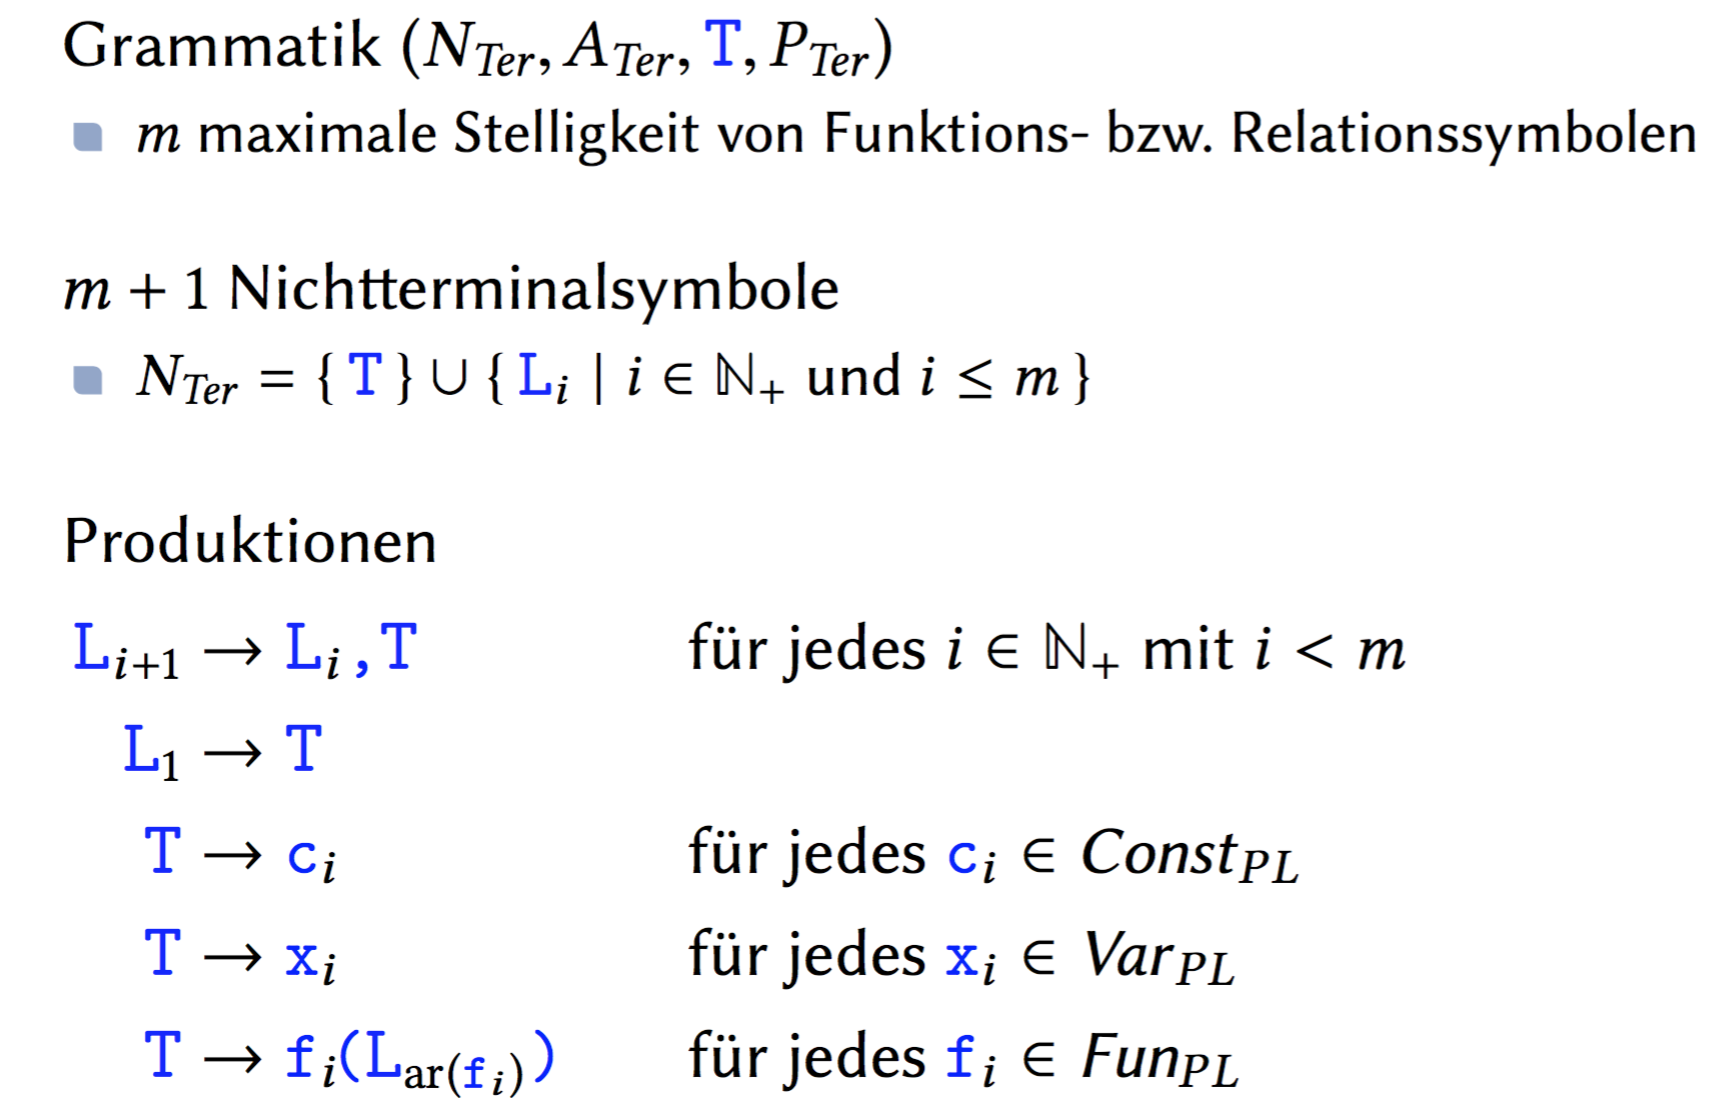
\includegraphics[scale=0.2]{pl/TermeGrammatik.png} \hspace{2em} 
\end{figure} 
\end{frame}

\begin{frame}{Atomare Formeln}
\begin{figure}[h!]
	\centering
	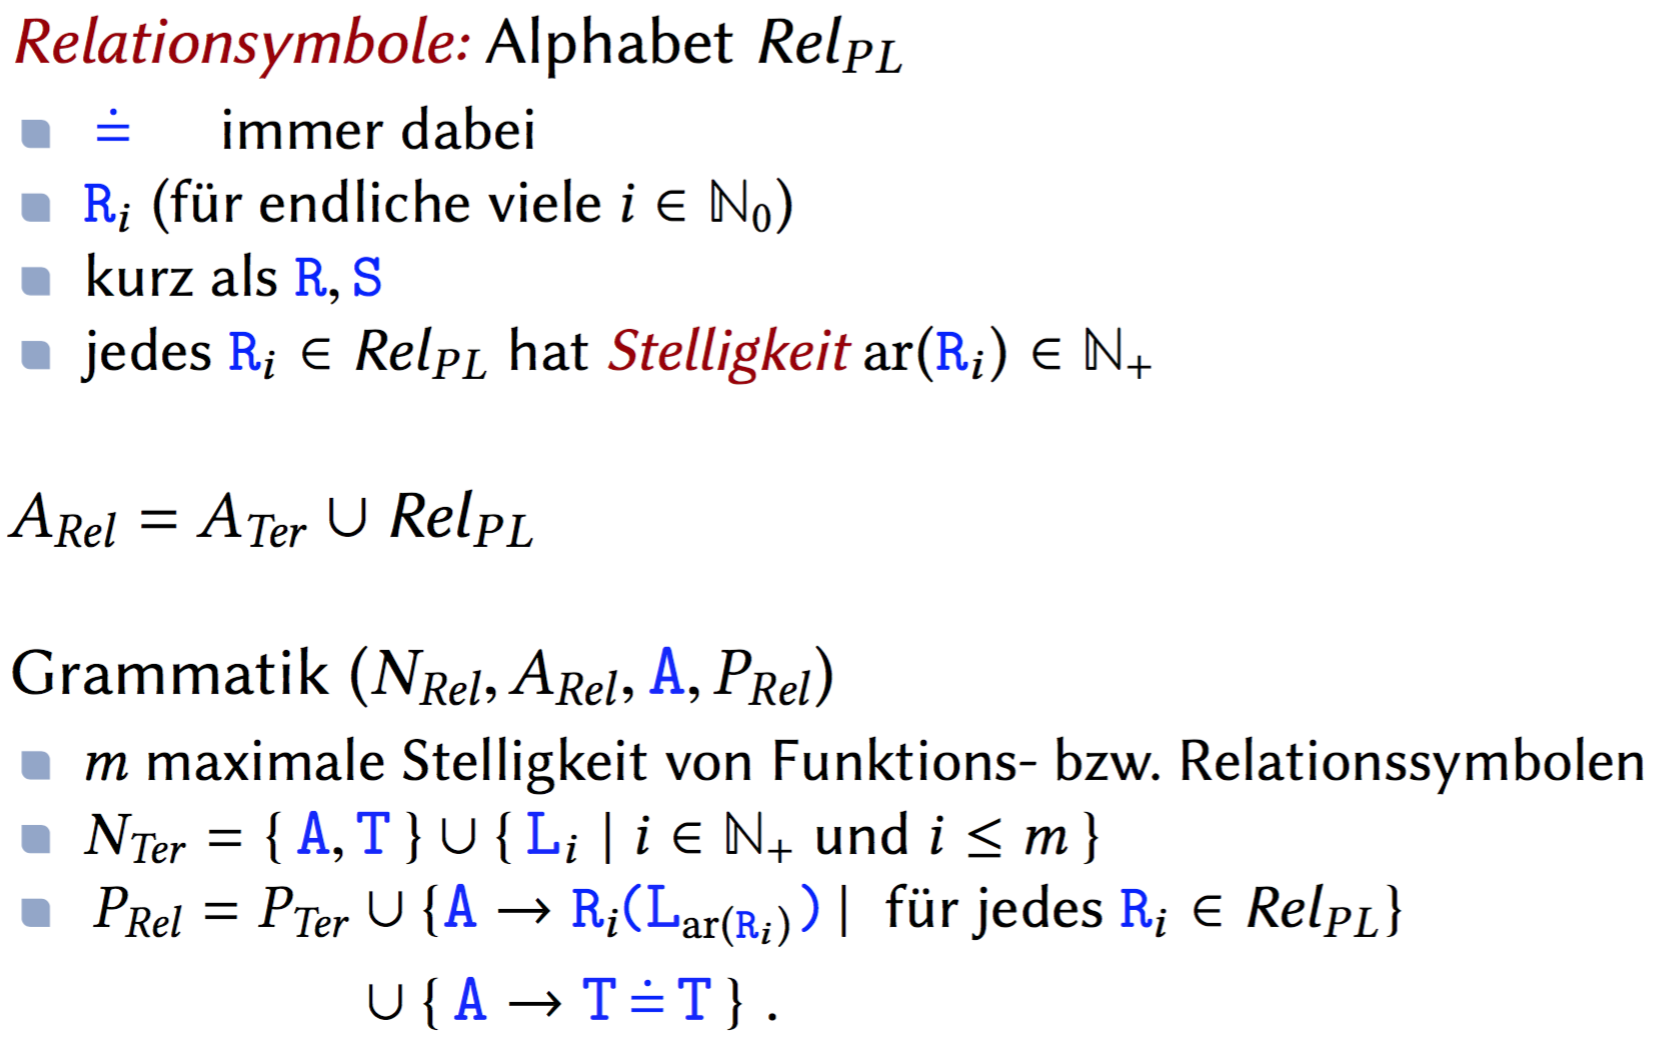
\includegraphics[scale=0.2]{pl/AFormeln.png} \hspace{2em} 
\end{figure} 
\end{frame}

\begin{frame}{Atomare Formeln - Beispiel}
\begin{figure}[h!]
	\centering
	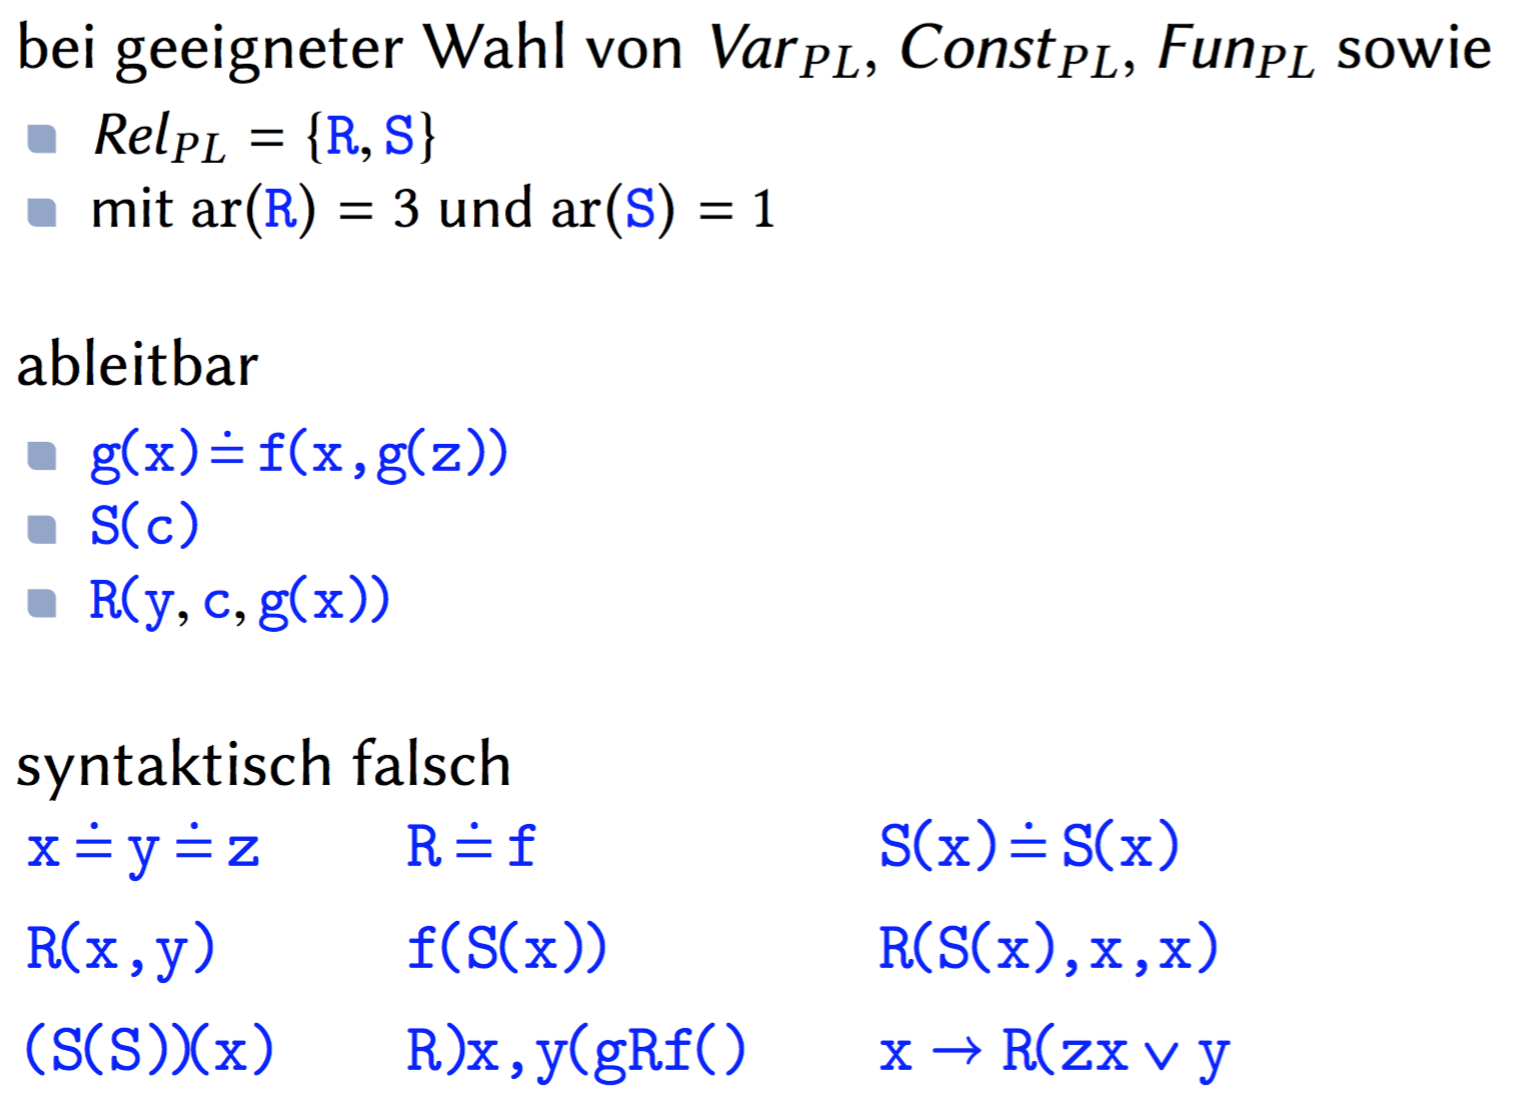
\includegraphics[scale=0.2]{pl/AFormelnBsp.png} \hspace{2em} 
\end{figure} 
\end{frame}

\begin{frame}{Prädikatenlogische Formeln}
\begin{figure}[h!]
	\centering
	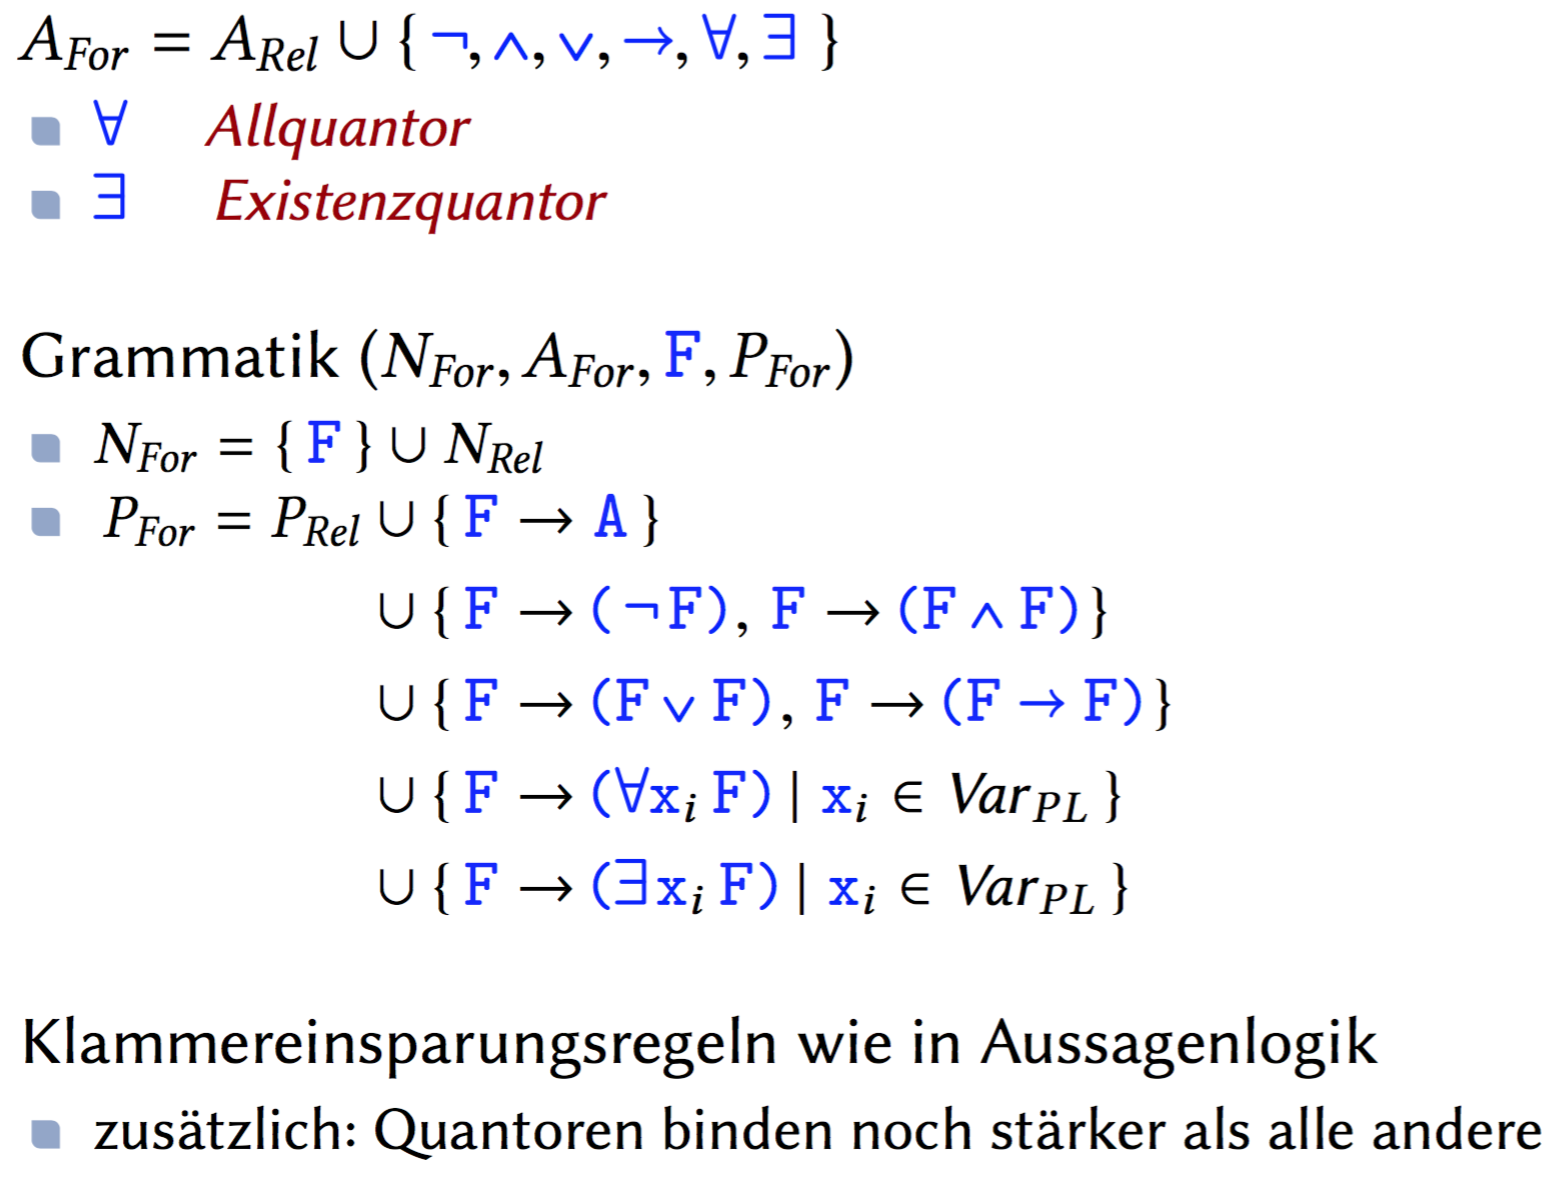
\includegraphics[scale=0.2]{pl/PFormeln.png} \hspace{2em} 
\end{figure} 
\end{frame}

\begin{frame}{Quiz}
\begin{figure}[h!]
	\centering
	\only<1|handout:1>{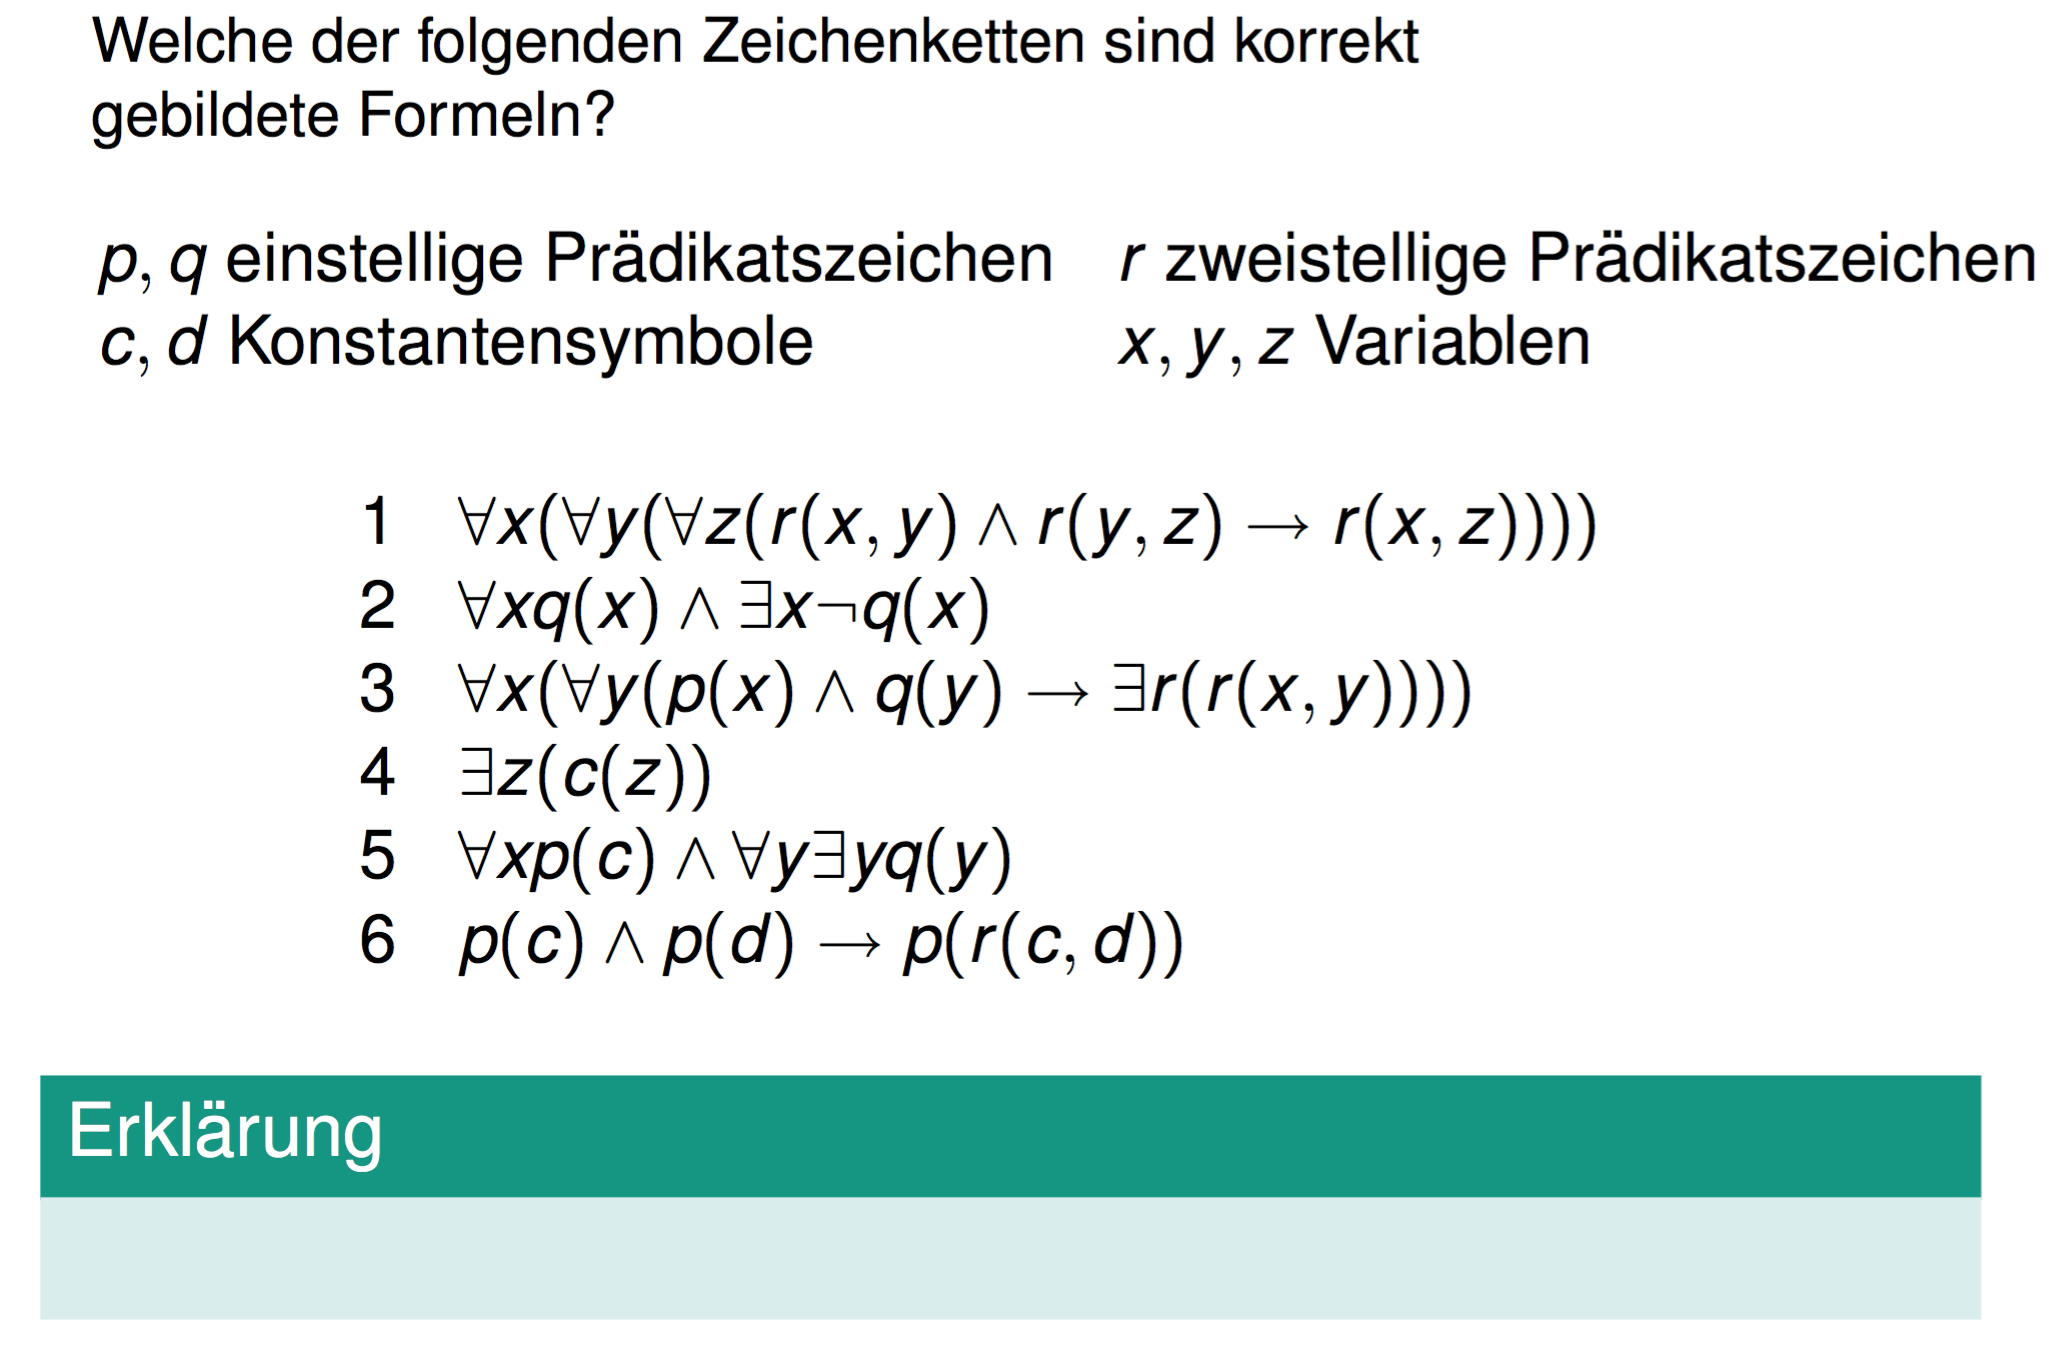
\includegraphics[scale=0.2]{pl/q1.png}}
	\only<2|handout:2>{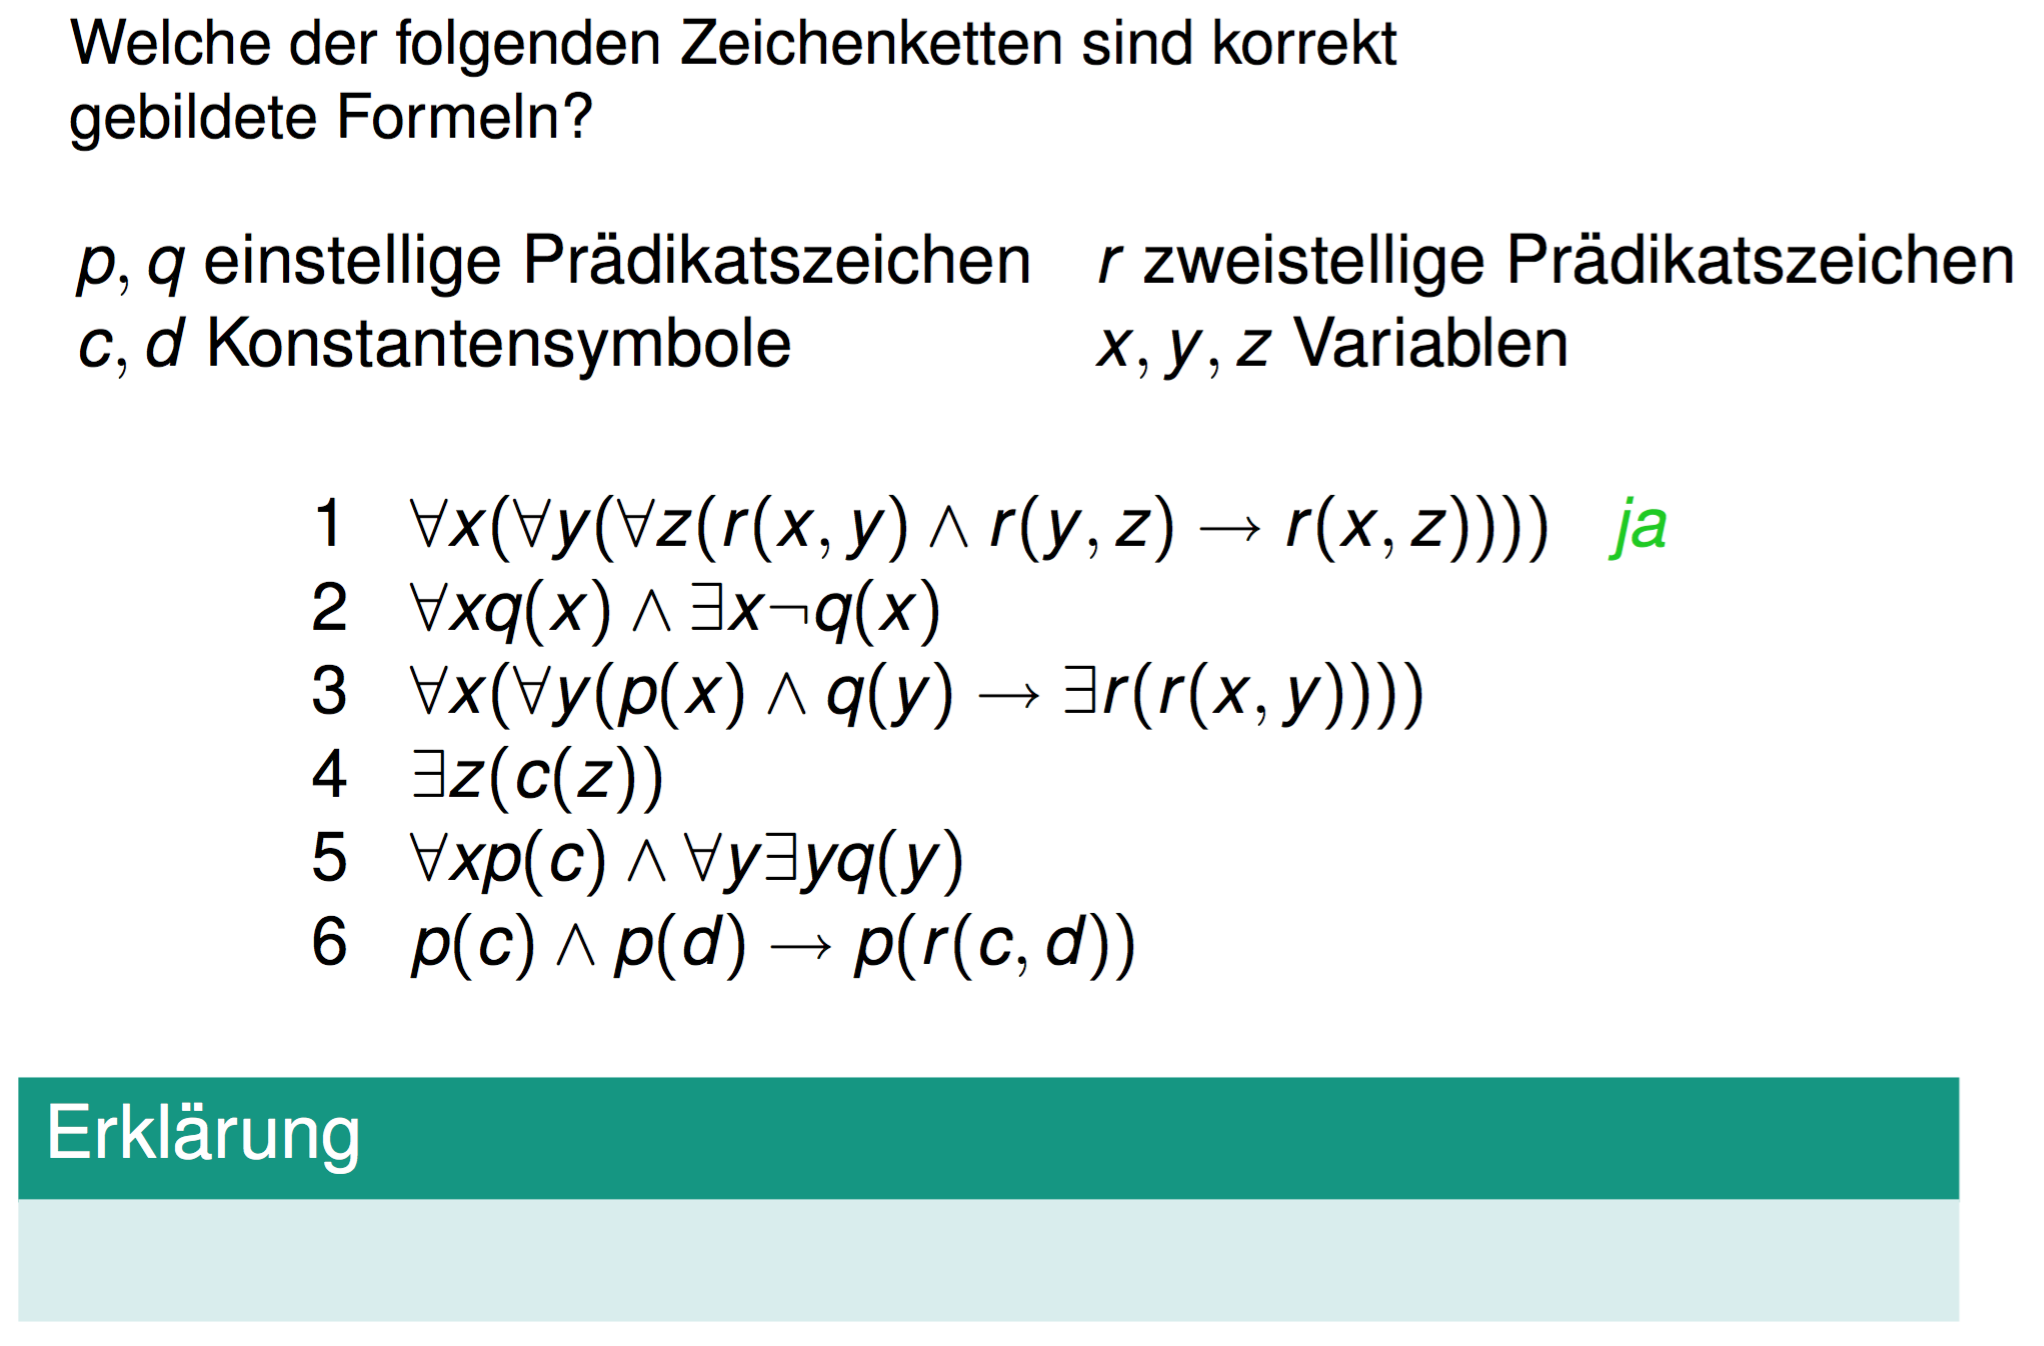
\includegraphics[scale=0.2]{pl/q2.png}} 
	\only<3|handout:3>{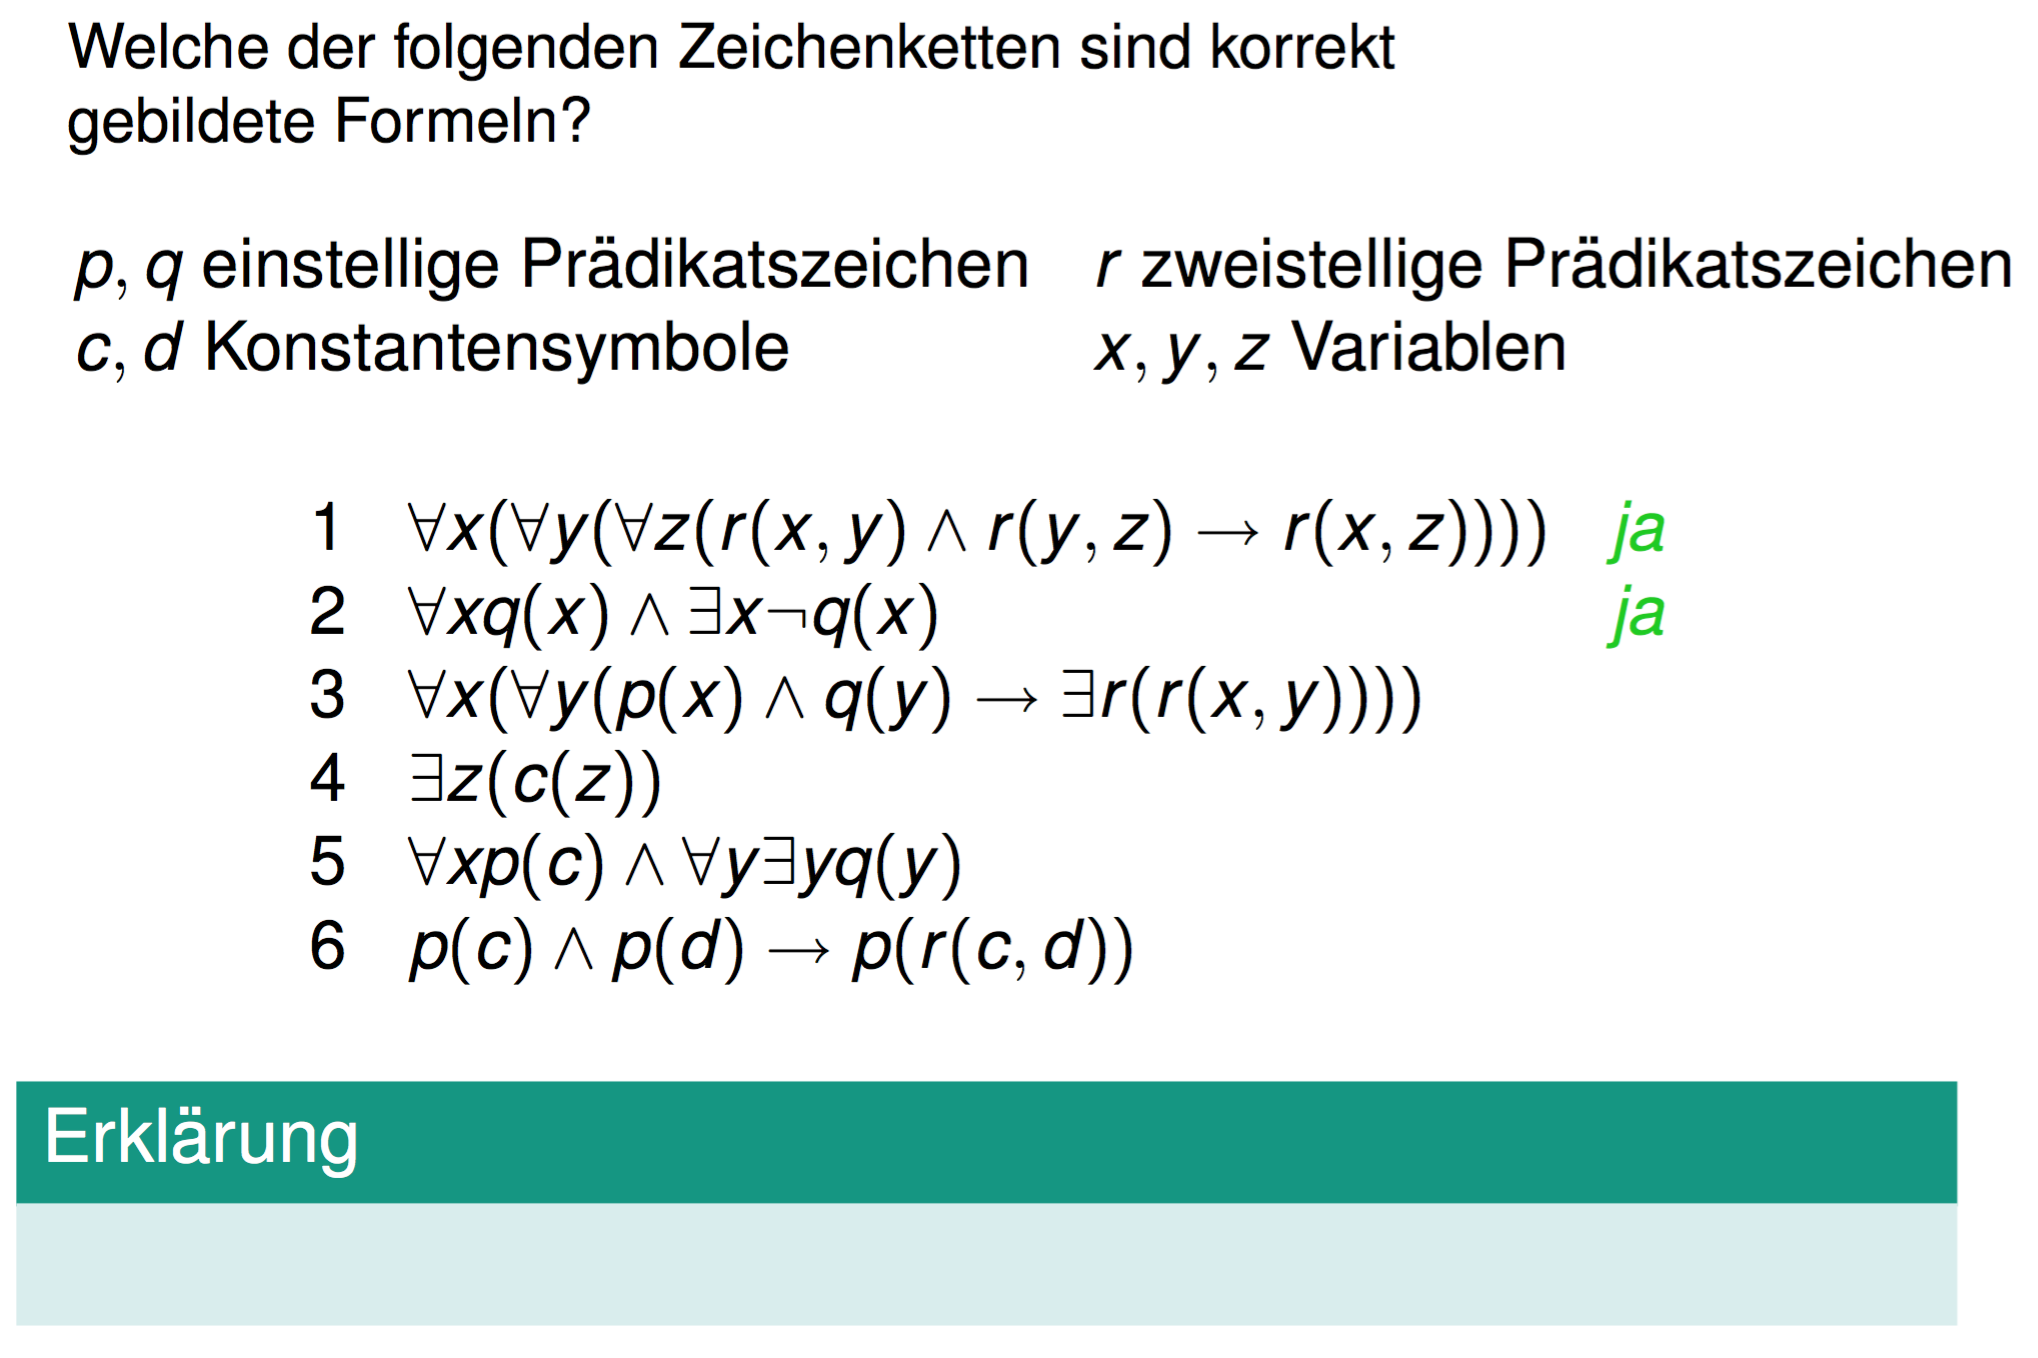
\includegraphics[scale=0.2]{pl/q3.png}}
	\only<4|handout:4>{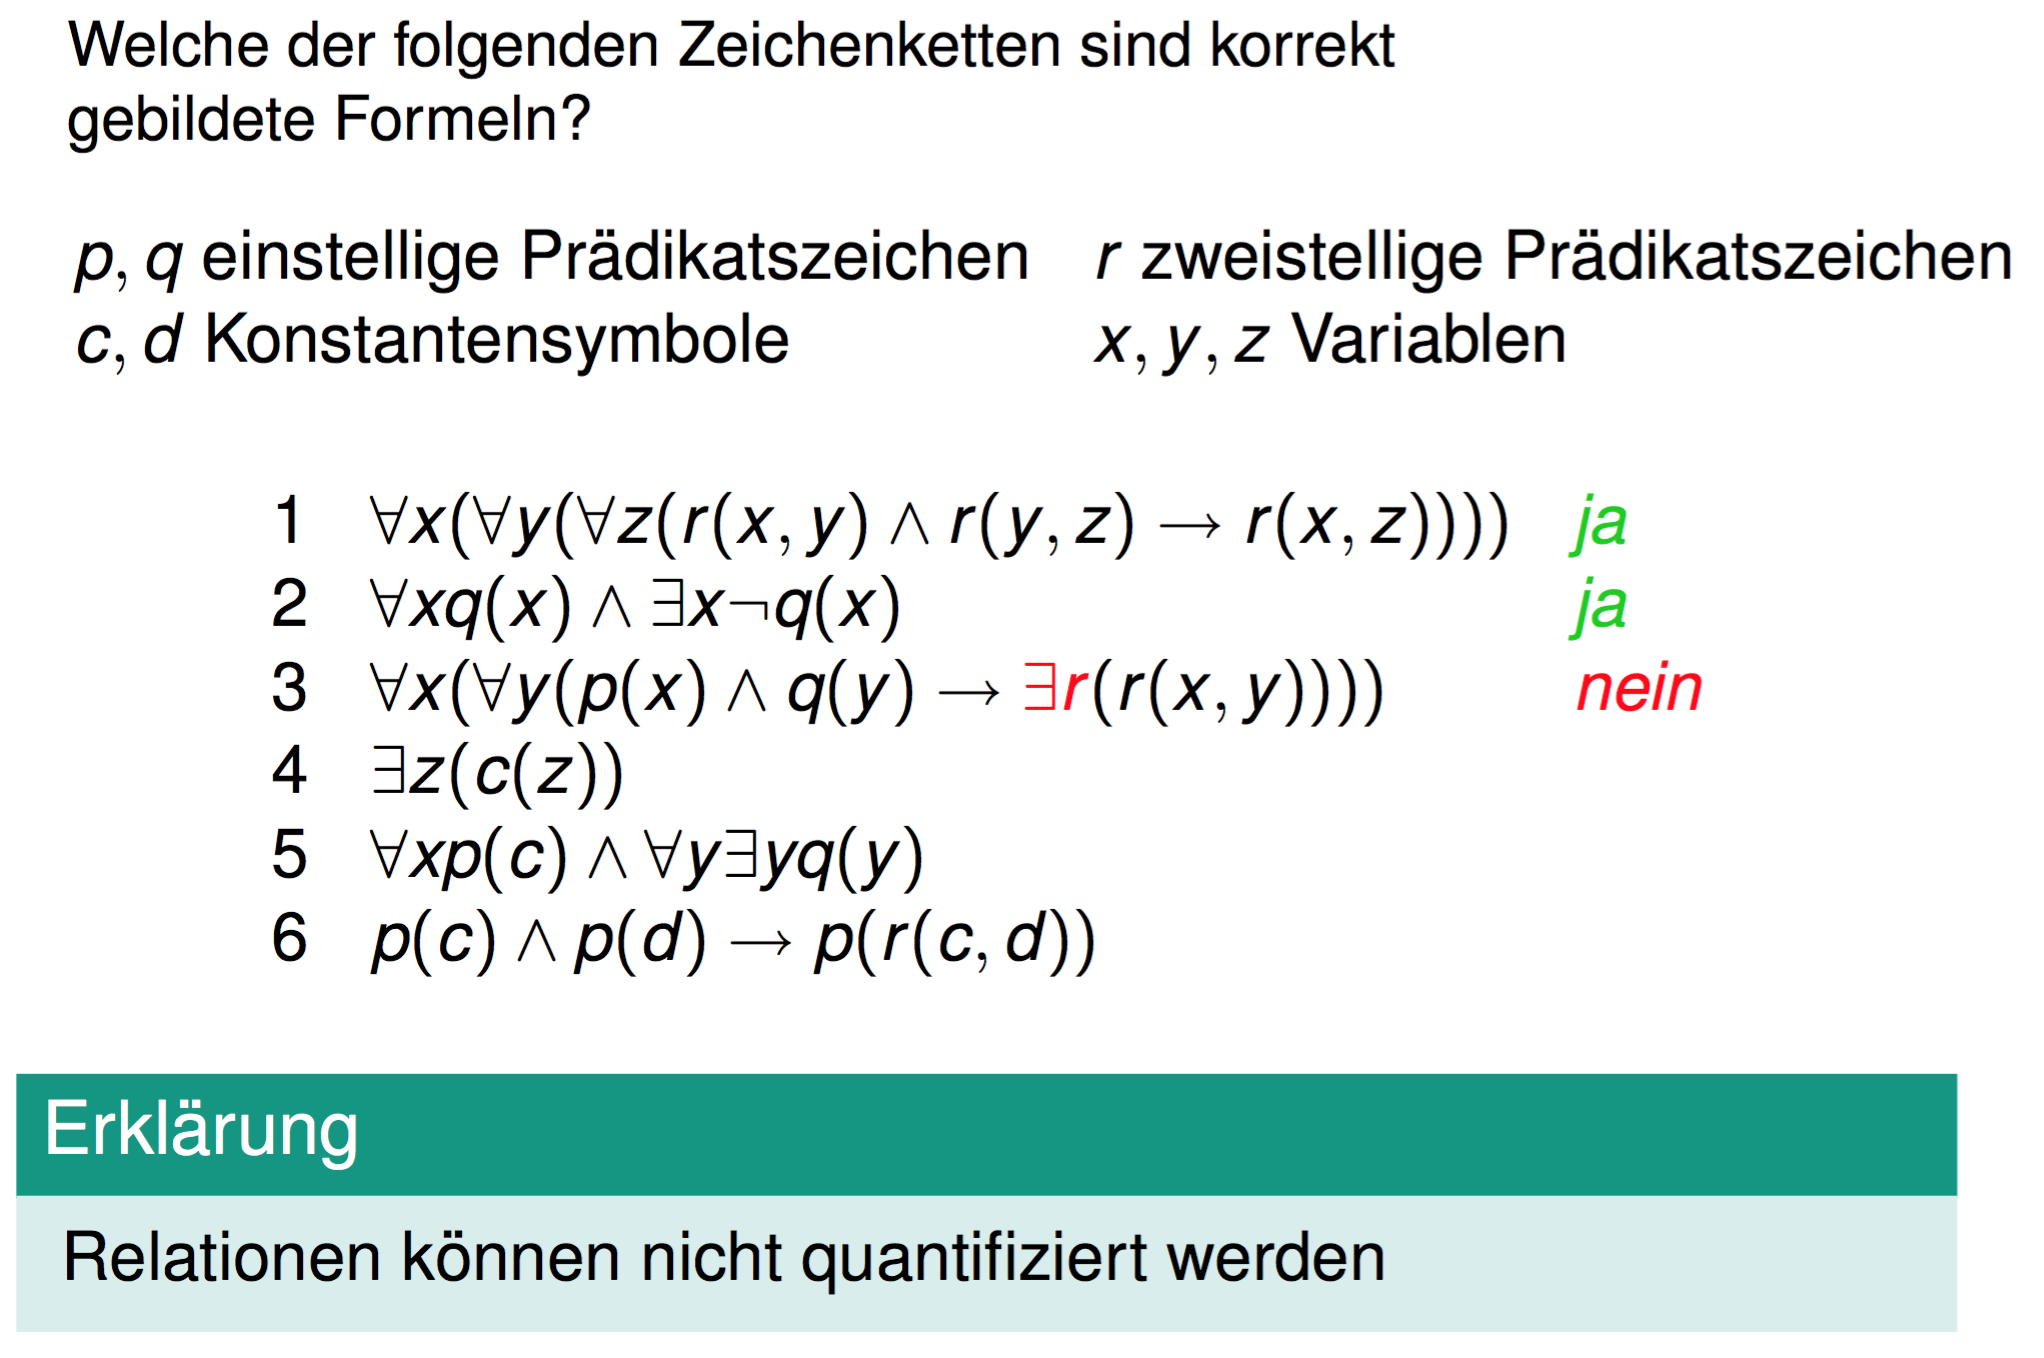
\includegraphics[scale=0.2]{pl/q4.png}}
	\only<5|handout:5>{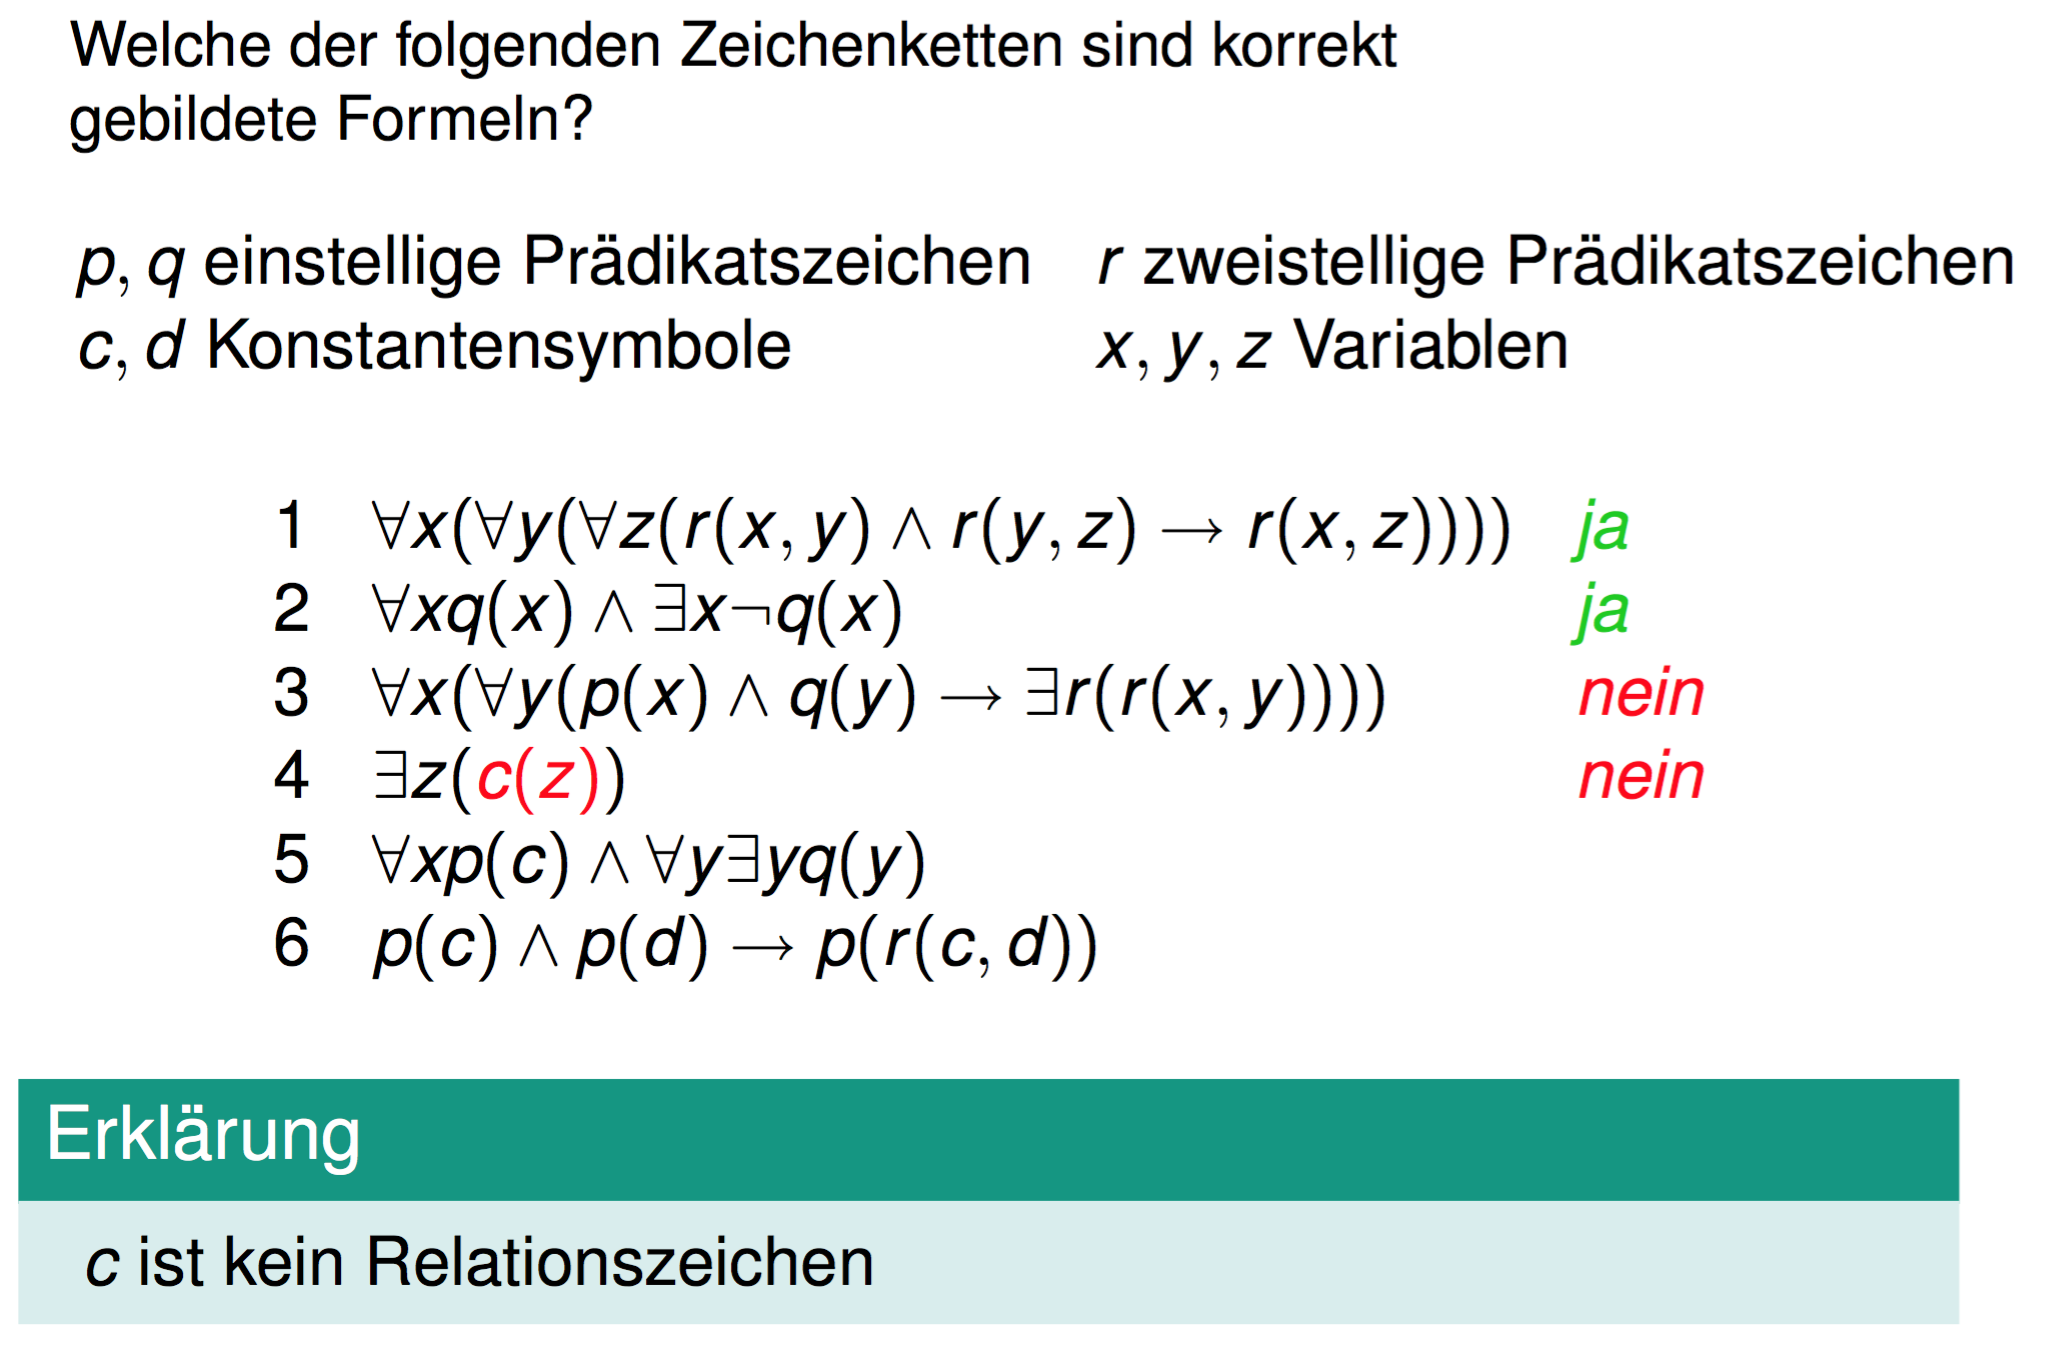
\includegraphics[scale=0.2]{pl/q5.png}}
	\only<6|handout:6>{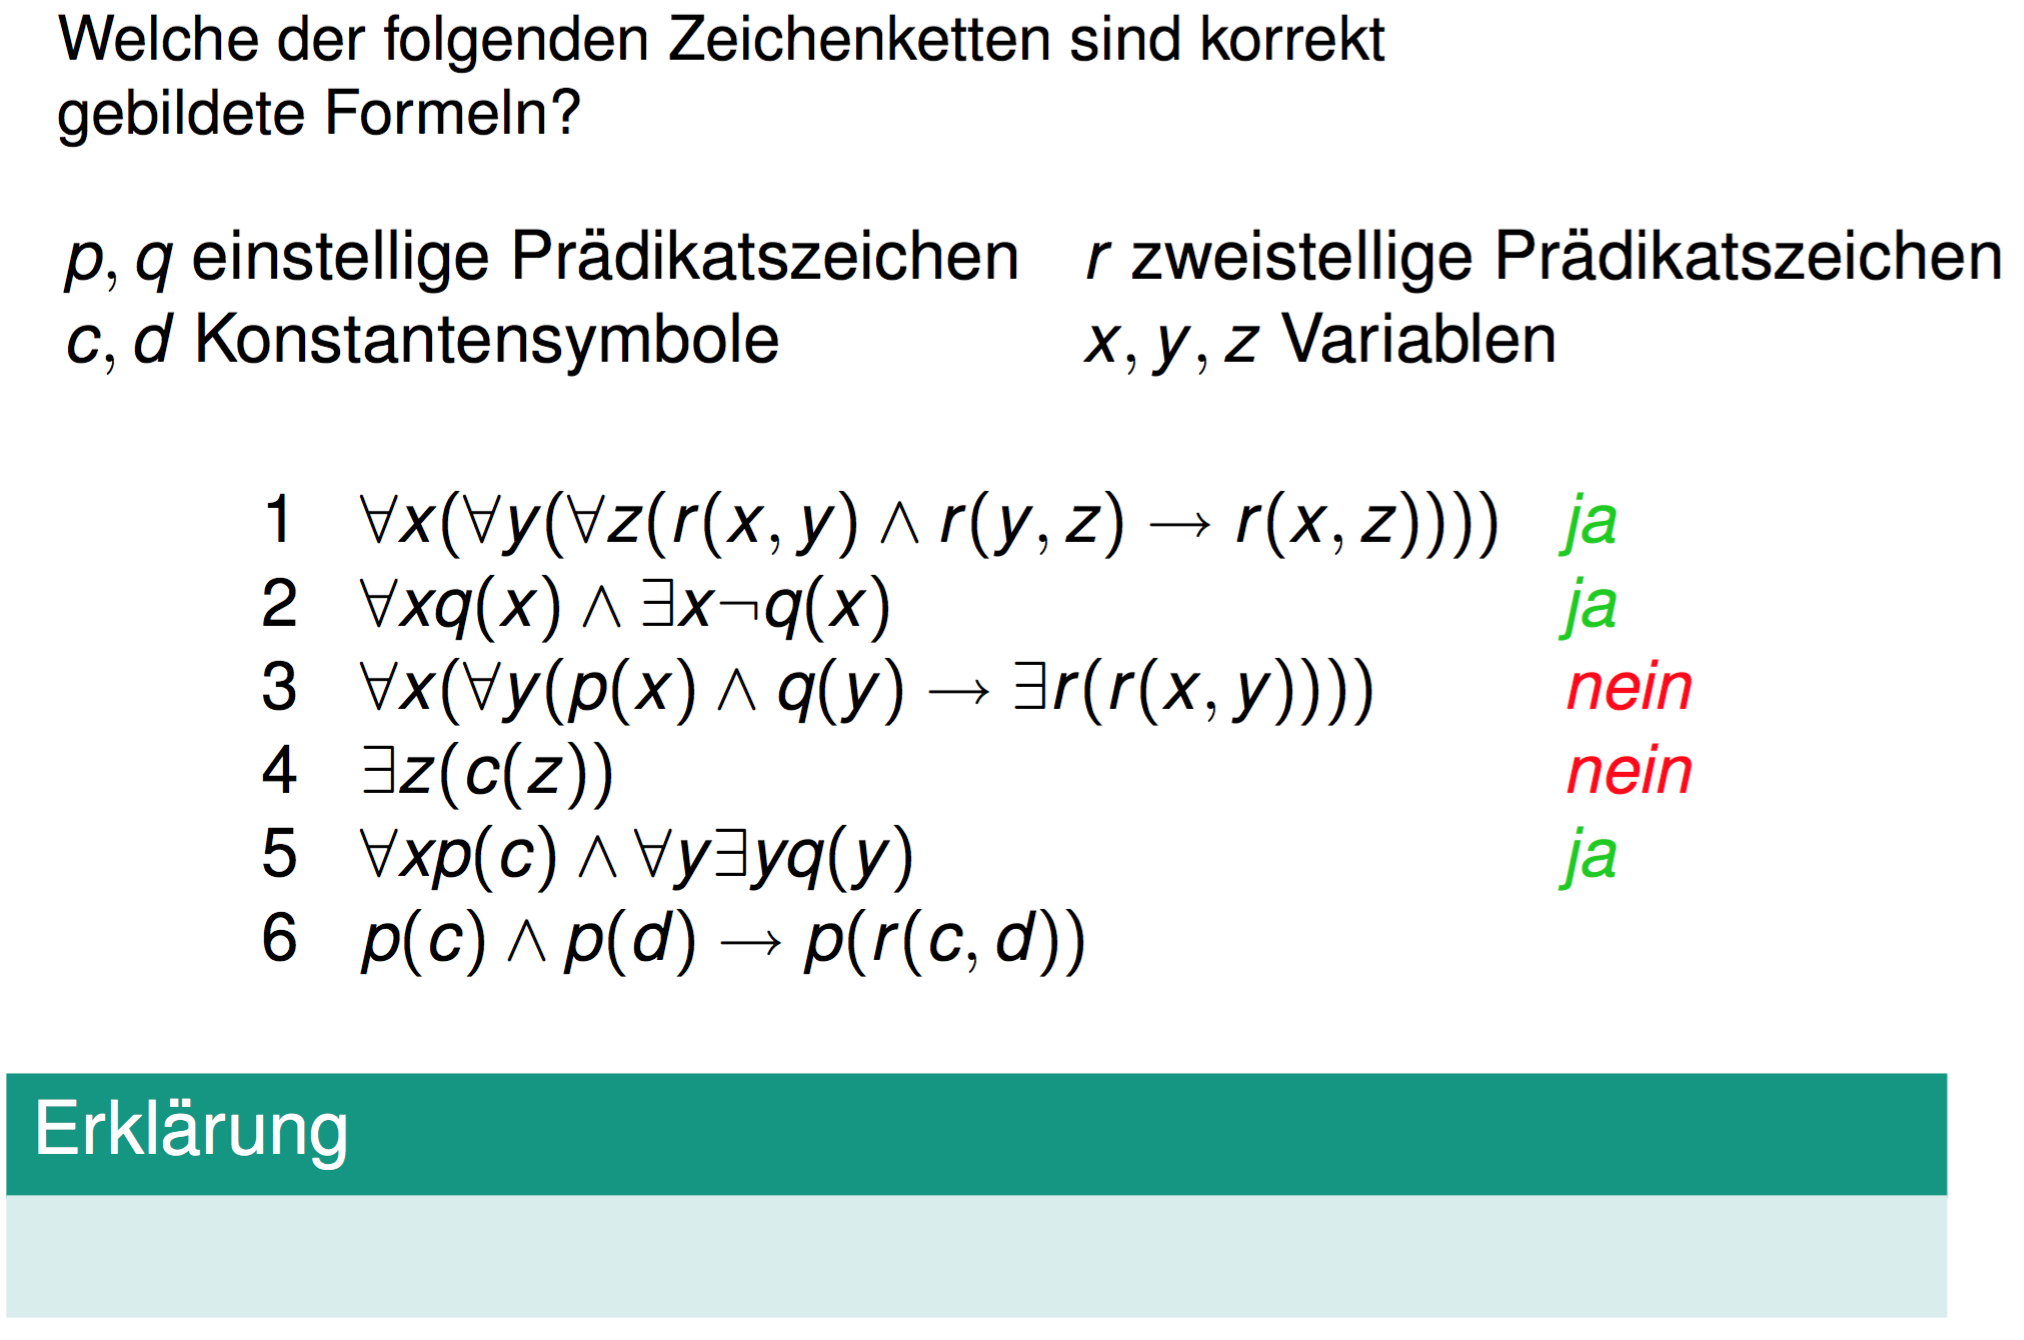
\includegraphics[scale=0.2]{pl/q6.png}}
	\only<7|handout:7>{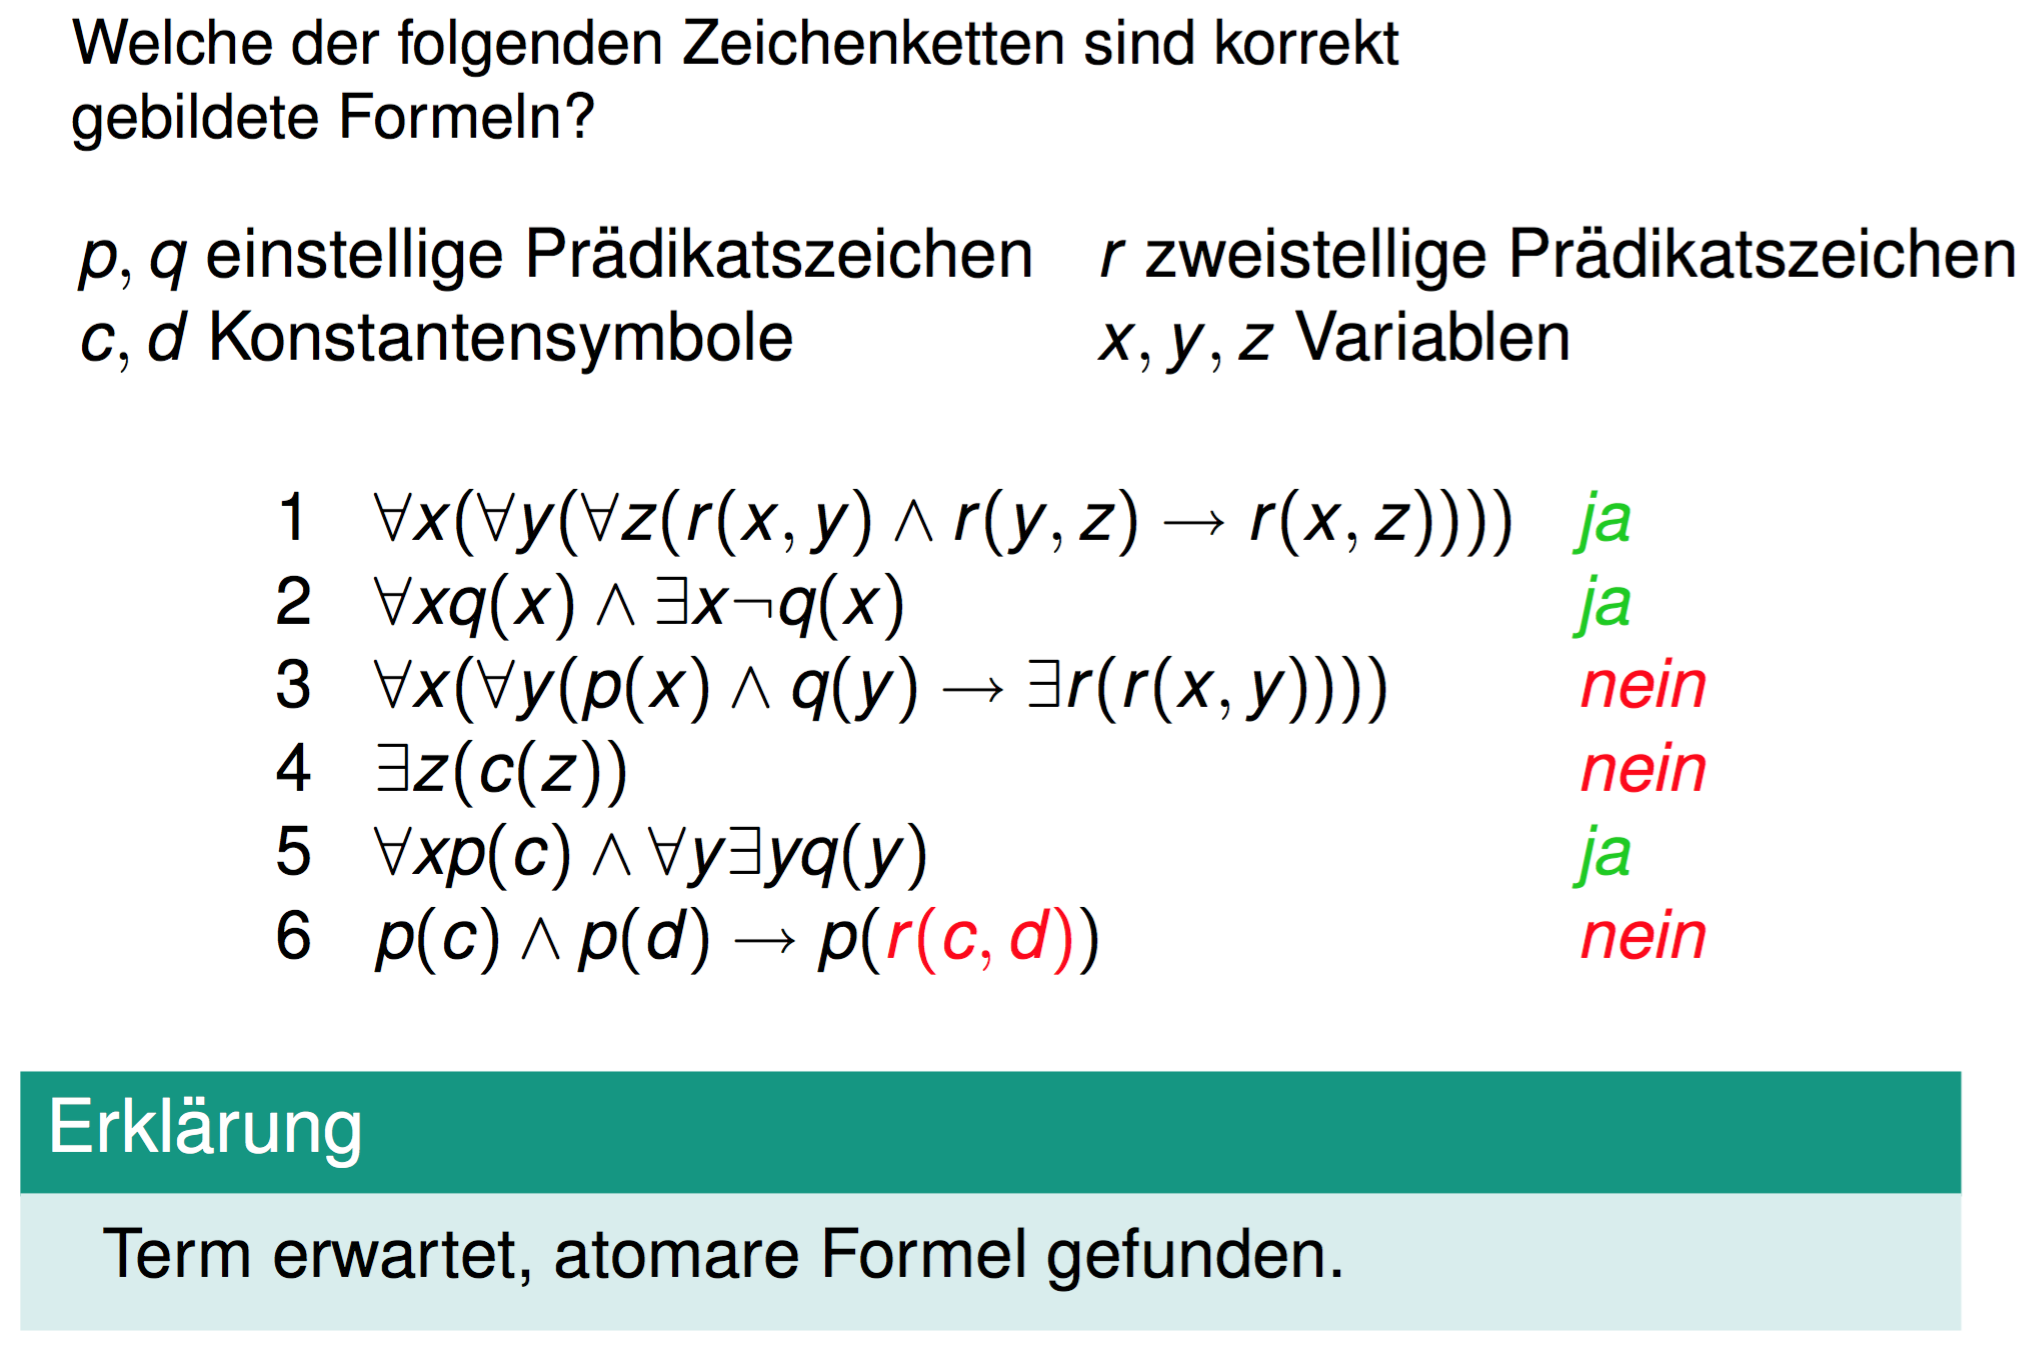
\includegraphics[scale=0.2]{pl/q7.png}}
	\hspace{2em}
\end{figure} 
\end{frame}

\begin{frame}{Freie und gebundene Variablenvorkommen}
	\begin{equation*}
	F = \alnot \plexist \plx
	{\plka
		\plE{\plka \plx \plcomma \ply \plkz}
		\alor
		\alnot \plall \plz \plall \plx \plall \ply
		{\plka
			\plE{\plka \plx \plcomma \plz \plkz} \aland \plE{\plka \ply \plcomma \plz \plkz} \alimpl \plx \pleq \ply
			\plkz}
		\plkz}
	\end{equation*}
	
	\begin{block}{Aufgabe 1.1}
		Welche Variablenvorkommen sind frei ($\fv$) und welche gebunden ($\bv$)?\\
		Ist die Formel geschlossen?
	\end{block}

	\pause
	\begin{block}{Lösung}
		Nur die Variable $\fv(F) = \{\ply\}$ kommt frei in $F$ vor.\\
		Genau die Variablen $\bv(F) = \{\plx, \ply, \plz\}$ kommen gebunden in $F$ vor.\\
		Da $\fv(F) \neq \emptyset$ ist $F$ nicht geschlossen.
	\end{block}
	
\end{frame}


\begin{frame}{Substitutionen}
	\begin{figure}[h!]
		\centering
		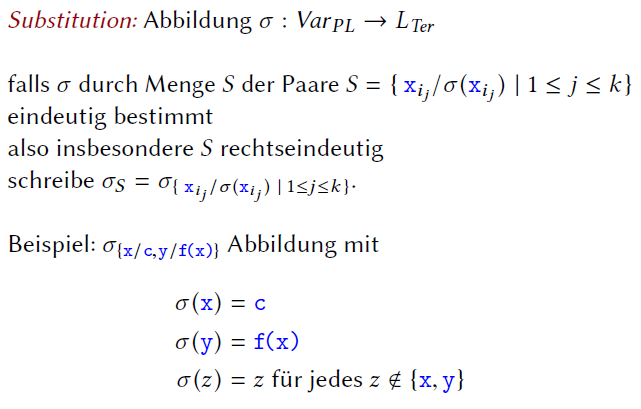
\includegraphics[scale=0.6]{pl/subs.png} \hspace{2em} 
	\end{figure} 
\end{frame}

\begin{frame}{Substitutionen}
	Ersetzt werden nur \textbf{freie Variablenvorkommen}!\\
	Gebundene Vorkommen, also Variablen im Wirkungsbereich eines Quantors, werden \textbf{nicht} ersetzt.
	
	\pause
	\begin{figure}[h!]
		\centering
		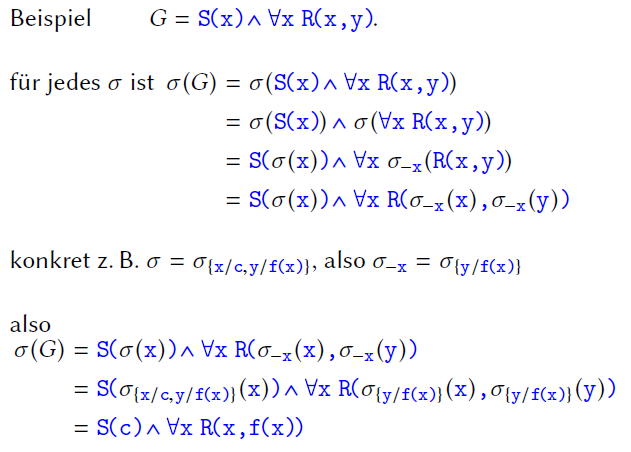
\includegraphics[scale=0.5]{pl/subs_bsp.png} \hspace{2em} 
	\end{figure} 
\end{frame}

\begin{frame}{Substitutionen: Kollisionsfreiheit}
	Bei einer \textbf{kollisionsfreien} Substitution werden keine Variablen \enquote{aus Versehen} gebunden.\\[1em]
	Ersetzen wir eine freie Variable $x$ durch einen Term, in dem die Variable $y$ frei vorkommt, so darf sich $x$ nicht im Wirkungsbereich eines Quantors über $y$ befinden.
	
	\pause
	\begin{Beispiel}
		$L = \plall \plx (\plx \aland \ply)$\\
		Kollisionsfrei: $\sigma_{\{\ply/\plz\}}$\\
		Nicht kollisionsfrei: $\sigma_{\{\ply/\plx\}}$
	\end{Beispiel}
\end{frame}

\begin{frame}{Substitutionen}
	\begin{equation*}
	F = \alnot \plexist \plx
	{\plka
		\plE{\plka \plx \plcomma \ply \plkz}
		\alor
		\alnot \plall \plz \plall \plx \plall \ply
		{\plka
			\plE{\plka \plx \plcomma \plz \plkz} \aland \plE{\plka \ply \plcomma \plz \plkz} \alimpl \plx \pleq \ply
			\plkz}
		\plkz}
	\end{equation*}
	
	\begin{block}{Aufgabe 1.2}
		Geben sie eine Substitution $\sigma$ an, die \emph{nicht} kollisionsfrei für $F$ ist.\\[1em] \pause
		
		Die Substitution $\sigma_{\{(\ply/\plx)\}}$ leistet das Gewünschte.
	\end{block}
	
\end{frame}


\section{Prädikatenlogik: Semantik}

\begin{frame}{Interpretation}
	\begin{figure}[h!]
		\centering
		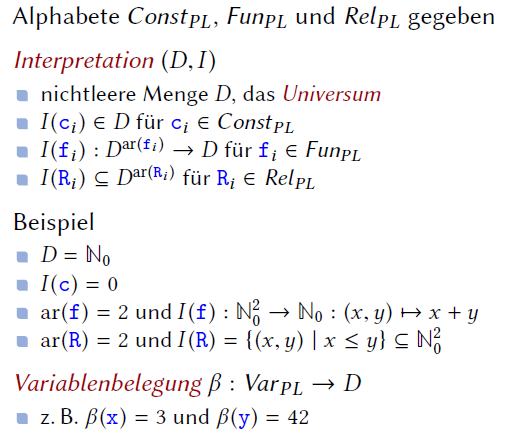
\includegraphics[scale=0.6]{pl/int.png} \hspace{2em} 
	\end{figure} 
\end{frame}

\begin{frame}{Aufgabe 1 (15/16, Blatt 7)}
	  \begin{equation*}
	\alnot \plexist \plx
	{\plka
		\plE{\plka \plx \plcomma \ply \plkz}
		\alor
		\alnot \plall \plz \plall \plx \plall \ply
		{\plka
			\plE{\plka \plx \plcomma \plz \plkz} \aland \plE{\plka \ply \plcomma \plz \plkz} \alimpl \plx \pleq \ply
			\plkz}
		\plkz}
	\end{equation*}\\[1em]
	
	\begin{block}{Aufgabe 1.3}
		Geben Sie eine Interpretation $(D_1, I_1)$ und eine Variablenbelegung $\beta_1$ so an, dass $val_{D_1, I_1, \beta_1}(F) = \textbf{W}$ gilt.\\[0.5em]
		
		\visible<2-|handout:2>{Die Interpretation $(D_1, I_1) = (\{ 0, 1 \}, {<})$ und die Variablenbelegung $\beta_1 \colon \VPL \to D$, $v \mapsto 0$, leisten das Gewünschte.}
	\end{block}

	\begin{block}{Aufgabe 1.4}
		Geben Sie eine Interpretation $(D_2, I_2)$ und eine Variablenbelegung $\beta_2$ so an, dass $val_{D_2, I_2, \beta_2}(F) = \textbf{F}$ gilt.\\[0.5em]
		
		\visible<3-|handout:2>{Die Interpretation $(D_2, I_2) = (\{ 0, 1 \}, {<})$ und die Variablenbelegung $\beta_2 \colon \VPL \to D$, $v \mapsto 1$, leisten das Gewünschte.}
	\end{block}
\end{frame}



\section{Prädikatenlogik: Aufgaben}

\begin{frame}{Prädikatenlogische Formeln aufstellen}
	% TODO Übung einbinden
	Vgl. Übung WS 15/16
\end{frame}

\begin{frame}{Aufgabe 2 (15/16, Blatt 7)}
	\begin{block}{Aufgabe}
		Formulieren Sie die folgenden Aussagen als Formeln in Prädikatenlogik:
		\begin{enumerate}
			\item Nicht alle Vögel können fliegen.
			\item Wenn es irgendjemand kann, dann kann es Donald Ervin Knuth.
			\item John liebt jeden, der sich nicht selbst liebt.
		\end{enumerate}
	\end{block}
	
	\only<2-|handout:2>{
	\begin{block}{Lösung}
		\begin{enumerate}
				\item
				\begin{equation*}
				\plexist \plx {\plka \plfoo{Vogel}{\plka \plx \plkz} \aland \alnot \plfoo{flugfaehig}{\plka \plx \plkz} \plkz}
				\end{equation*}
			\only<3-|handout:2>{
				\item
				\begin{equation*}
				\plexist \plx {\plka \plfoo{kann\_es}{\plka \plx \plkz} \plkz}
				\alimpl
				\plfoo{kann\_es}{\plka \plfoo{knuth} \plkz}
				\end{equation*}
			}
			\only<4-|handout:2>{
				\item
				\begin{equation*}
				\plall \plx {\plka \alnot \plfoo{liebt}{\plka \plx \plcomma \plx \plkz} \alimpl \plfoo{liebt}{\plka \plfoo{John} \plcomma \plx \plkz} \plkz}
				\end{equation*}
			}
		\end{enumerate}
	\end{block}
	}
\end{frame}

\begin{frame}{Weitere Aufgaben}
	Siehe Übung WS 15/16
\end{frame}